\documentclass[12pt]{article}
\usepackage{amsmath}
\usepackage{tikz}
\begin{document}
\title{Computer Science 181, Homework 7}
\date{May 21st, 2018}
\author{Michael Wu\\UID: 404751542}
\maketitle

\section*{Problem 0}

The language \(L_0\) is context free and not finite state. The context free grammar \(G\) that describes the language is shown below.
\begin{align*}
        G&=(V,\Sigma,R,S)\\
        V&=\{A,B,C,D,T\}\\
        R&=\{T\rightarrow AB \mid CD,\\
        &\hphantom{==}A\rightarrow \text{a}A\text{b} \mid \epsilon,\\
        &\hphantom{==}B\rightarrow \text{c}B \mid \epsilon,\\
        &\hphantom{==}C\rightarrow \text{a}C \mid \epsilon,\\
        &\hphantom{==}D\rightarrow \text{b}D\text{c} \mid \epsilon\}\\
        S&=T
\end{align*}
To prove that \(L_0\) is not finite state, first assume for contradiction that \(L_0\) is finite state. Then by the pumping lemma for finite state languages,
there exists some \(p\) such that \(\forall w\in L_0\) with \(|w|\geq p\), \(w\) can be split into three substrings \(x\), \(y\), and \(z\) such that \(w=xyz\),
\(|y|\geq 1\), \(|xy|\leq p\), and \(\forall n\geq 0\) we have that \(xy^nz\in L_0\). But consider the string \(w=\text{b}^p\text{c}^p\), which is in \(L_0\)
and has a length greater than \(p\). When splitting \(w\) into \(x\), \(y\), and \(z\), because \(|xy|\leq p\), we have that \(x\) and \(y\) must consist
entirely of b's. We know that \(|y|\geq 1\), so for any \(n\geq 2\) we have that \(xy^nz\) must take the form \(\text{b}^i\text{c}^j\) with \(i>j\). This
is not in the language \(L_0\), which is a contradiction. Thus \(L_0\) is not a finite state language.

\section*{Problem 1}

The language \(L_1\) is context free and not finite state. The PDA with the set of stack symbols \(\Gamma = \{a\}\) is shown below.
\begin{center}
        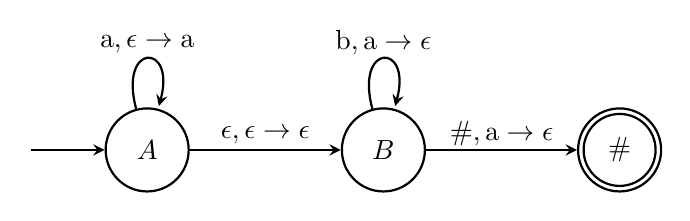
\begin{tikzpicture}
                \begin{scope}[auto, every node/.style={thick, draw,circle,minimum size=3em,inner sep=1}]
                        \node (A) at (0,0) {\(A\)};
                        \node (B) at (3,0) {\(B\)};
                        \node (Hash) at (6,0) {\#};
                        \draw[black, thick] (6,0) circle [radius=1.3em];
                \end{scope}
                \node [draw=none, inner sep=0pt] (I) at (-1.5,0) {};
                \begin{scope}[auto, every node/.style={minimum size=1em,inner sep=1}, every path/.style={thick, ->, >=stealth}]
                        \path (I) edge (A);
                        \path (A) edge [loop above] node {\(\text{a}, \epsilon\rightarrow\text{a}\)} (A);
                        \path (A) edge node {\(\epsilon, \epsilon\rightarrow\epsilon\)} (B);
                        \path (B) edge [loop above] node {\(\text{b}, \text{a}\rightarrow\epsilon\)}(B);
                        \path (B) edge node {\(\text{\#}, \text{a}\rightarrow\epsilon\)} (Hash);
                \end{scope}
        \end{tikzpicture}
\end{center}
To prove that \(L_1\) is not finite state, first assume for contradiction that \(L_1\) is finite state. Then by the pumping lemma for finite state languages,
there exists some \(p\) such that \(\forall w\in L_1\) with \(|w|\geq p\), \(w\) can be split into three substrings \(x\), \(y\), and \(z\) such that \(w=xyz\),
\(|y|\geq 1\), \(|xy|\leq p\), and \(\forall n\geq 0\) we have that \(xy^nz\in L_1\). But consider the string \(w=\text{a}^i\text{b}^j\text{\#}\) in \(L_1\)
such that \(i+j\geq p\) and \(i=j+1\). Because \(|xy|\leq p\) when splitting \(w\) into the three substrings, \(y\) can only be chosen such that it consists
entirely of a's, entirely of b's, or contains a sequence of a's followed by a sequence of b's. If \(y\) consists entirely of a's then the string \(xy^nz\)
with \(n=0\) will not be in \(L_1\), as this will result in an equal or lesser amount of a's than b's in the string. So \(y\) cannot consist entirely of a's.
If \(y\) consists entirely of b's then the string \(xy^nz\) with \(n\geq 2\) will not be in \(L_1\), as this will result in an equal or greater amount of b's
than a's in the string. So \(y\) cannot consist entirely of b's. If \(y\) consists of a sequence of a's followed by a sequence of b's, then the string \(xy^nz\)
with \(n\geq 2\) will not be in \(L_1\), as this string will have interleaved a's and b's, which does not fit the format of \(\text{a}^i\text{b}^j\text{\#}\).
So \(y\) cannot consist of a sequence of a's followed by a sequence of b's. Thus there exists some \(w \in L_1\) with \(|w|\geq p\) that cannot be split into
three substrings \(x\), \(y\), and \(z\) such that \(w=xyz\), \(|y|\geq 1\), \(|xy|\leq p\), and \(\forall n\geq 0\) we have that \(xy^nz\in L_1\). This is a
contradiction, and so \(L_1\) cannot be finite state.

\section*{Problem 2}

Assume for contradiction that \(L_2\) is a context free language. Then by the pumping lemma for context free languages, there exists some
\(p\) such that \(\forall s\in L_2\) with \(|s|\geq p\), \(s\) can be split into five substrings \(u\), \(v\), \(w\), \(x\), and \(y\) such that
\(|vwx|\leq p\), \(|vx|\geq 1\), and \(\forall n\geq 0\) we have that \(uv^nwx^ny\in L_2\). Consider the string \(s=t\#t^R\#t\) in \(L_2\), with \(|t|\geq p\).
Then when attempting to split \(s\), \(vwx\) can only contain one or zero \#'s because \(|vwx|\leq p\), which means \(vx\) can contain only one or zero \#'s.
If \(vx\) contains one \#, then \(uv^nwx^ny\) would contain three \#'s for \(n=2\), and thus \(uv^nwx^ny\) would not be in \(L_2\) since it does not fit the
format of \(t\#t^R\#t\). If \(vx\) contains zero \#'s, then \(w\) contains either one or zero \#'s. If \(w\) contains zero \#'s and \(vx\) contains zero \#'s,
then \(v\) and \(x\) must lie entirely within one \(t\) or within the \(t^R\). Thus \(uv^nwx^ny\) will be in the form \(r\#t^R\#t\), \(t\#r^R\#t\), or \(t\#t^R\#r\)
with \(r\neq t\) for \(n\geq 2\). Then \(uv^nwx^ny\) would not be in \(L_2\). If \(w\) contains one \#, then \(uv^nwx^ny\) will be in the form \(q\#r^R\#t\) or
\(t\#q^R\#r\) with \(q\neq t\) and \(r\neq t\) for \(n\geq 2\). Then \(uv^nwx^ny\) would not be in \(L_2\). So there exists some string \(s\) such that \(s\) cannot be
split into five substrings that make the conditions of the pumping lemma hold. This is a contradiction, and thus \(L_2\) is not a context free language.

\end{document}